\documentclass{standalone}
\usepackage{tikz}
\usetikzlibrary{patterns, positioning}

\begin{document}
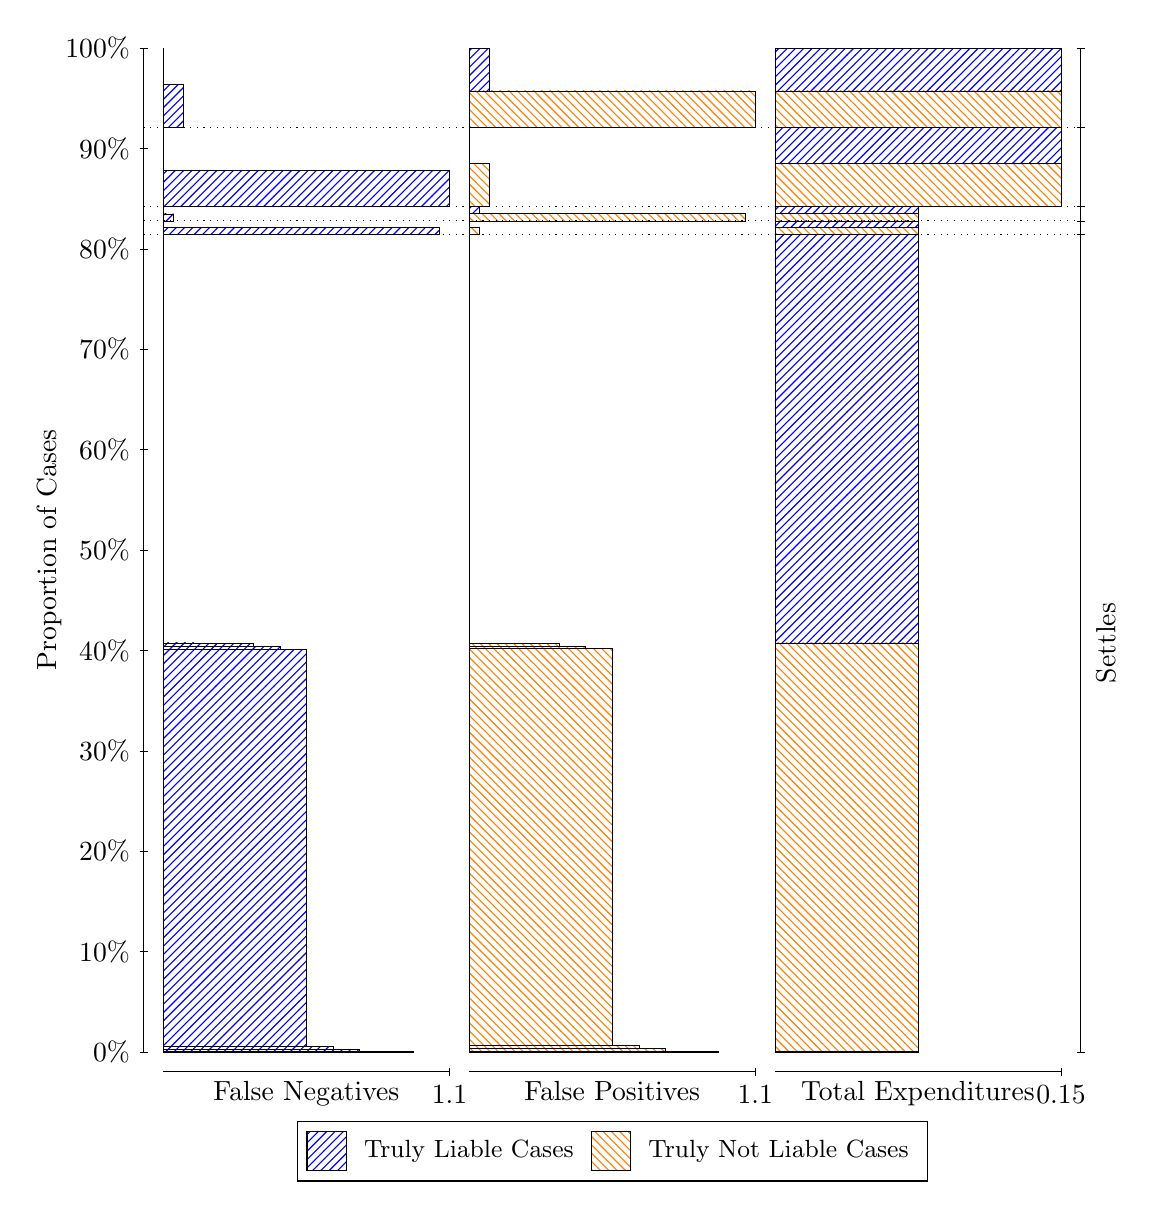
\begin{tikzpicture}
\draw[black, very thin] (1.5,1.75) -- (1.5,14.5);
\node[rotate=90, anchor=center] at (0.3, 8.125) {Proportion of Cases};
\draw[black, very thin] (1.45,1.75) -- (1.55,1.75);
\node[anchor=east] at (1.45, 1.75) {0\%};
\draw[black, very thin] (1.45,3.025) -- (1.55,3.025);
\node[anchor=east] at (1.45, 3.025) {10\%};
\draw[black, very thin] (1.45,4.3) -- (1.55,4.3);
\node[anchor=east] at (1.45, 4.3) {20\%};
\draw[black, very thin] (1.45,5.575) -- (1.55,5.575);
\node[anchor=east] at (1.45, 5.575) {30\%};
\draw[black, very thin] (1.45,6.85) -- (1.55,6.85);
\node[anchor=east] at (1.45, 6.85) {40\%};
\draw[black, very thin] (1.45,8.125) -- (1.55,8.125);
\node[anchor=east] at (1.45, 8.125) {50\%};
\draw[black, very thin] (1.45,9.4) -- (1.55,9.4);
\node[anchor=east] at (1.45, 9.4) {60\%};
\draw[black, very thin] (1.45,10.675) -- (1.55,10.675);
\node[anchor=east] at (1.45, 10.675) {70\%};
\draw[black, very thin] (1.45,11.95) -- (1.55,11.95);
\node[anchor=east] at (1.45, 11.95) {80\%};
\draw[black, very thin] (1.45,13.225) -- (1.55,13.225);
\node[anchor=east] at (1.45, 13.225) {90\%};
\draw[black, very thin] (1.45,14.5) -- (1.55,14.5);
\node[anchor=east] at (1.45, 14.5) {100\%};

\draw[black, very thin] (13.4,1.75) -- (13.4,14.5);
\draw[black, very thin] (13.35,1.75) -- (13.45,1.75);
\node[anchor=west] at (13.35, 1.75) {};
\draw[black, very thin] (13.35,12.136) -- (13.45,12.136);
\node[anchor=west] at (13.35, 12.136) {};
\draw[black, very thin] (13.35,12.306) -- (13.45,12.306);
\node[anchor=west] at (13.35, 12.306) {};
\draw[black, very thin] (13.35,12.487) -- (13.45,12.487);
\node[anchor=west] at (13.35, 12.487) {};
\draw[black, very thin] (13.35,13.493) -- (13.45,13.493);
\node[anchor=west] at (13.35, 13.493) {};
\draw[black, very thin] (13.35,14.5) -- (13.45,14.5);
\node[anchor=west] at (13.35, 14.5) {};

\draw[black, very thin, pattern color=blue, pattern=north east lines] (1.75,1.75) rectangle (4.9186,1.7536);
\draw[black, very thin, pattern color=blue, pattern=north east lines] (1.75,1.7536) rectangle (4.5806,1.7539);
\draw[black, very thin, pattern color=blue, pattern=north east lines] (1.75,1.7539) rectangle (4.2426,1.7873);
\draw[black, very thin, pattern color=blue, pattern=north east lines] (1.75,1.7873) rectangle (3.9047,1.8207);
\draw[black, very thin, pattern color=blue, pattern=north east lines] (1.75,1.8207) rectangle (3.5667,6.8675);
\draw[black, very thin, pattern color=blue, pattern=north east lines] (1.75,6.8675) rectangle (3.2287,6.9037);
\draw[black, very thin, pattern color=blue, pattern=north east lines] (1.75,6.9037) rectangle (2.8907,6.9406);
\draw[black, very thin, pattern color=blue, pattern=north east lines] (1.75,6.9406) rectangle (2.5527,6.9417);
\draw[black, very thin, pattern color=blue, pattern=north east lines] (1.75,6.9417) rectangle (2.2147,6.9443);
\draw[black, very thin, pattern color=orange, pattern=north west lines] (1.75,6.9443) rectangle (1.75,12.136);
\draw[black, very thin, pattern color=blue, pattern=north east lines] (1.75,12.136) rectangle (5.2566,12.221);
\draw[black, very thin, pattern color=orange, pattern=north west lines] (1.75,12.221) rectangle (1.75,12.306);
\draw[black, very thin, pattern color=blue, pattern=north east lines] (1.75,12.306) rectangle (1.8767,12.395);
\draw[black, very thin, pattern color=orange, pattern=north west lines] (1.75,12.395) rectangle (1.75,12.487);
\draw[black, very thin, pattern color=blue, pattern=north east lines] (1.75,12.487) rectangle (5.3833,12.95);
\draw[black, very thin, pattern color=orange, pattern=north west lines] (1.75,12.95) rectangle (1.75,13.493);
\draw[black, very thin, pattern color=blue, pattern=north east lines] (1.75,13.493) rectangle (2.0035,14.038);
\draw[black, very thin, pattern color=orange, pattern=north west lines] (1.75,14.038) rectangle (1.75,14.5);
\draw[black, very thin, pattern color=orange, pattern=north west lines] (5.6333,1.75) rectangle (8.8019,1.7527);
\draw[black, very thin, pattern color=orange, pattern=north west lines] (5.6333,1.7527) rectangle (8.464,1.7539);
\draw[black, very thin, pattern color=orange, pattern=north west lines] (5.6333,1.7539) rectangle (8.126,1.7926);
\draw[black, very thin, pattern color=orange, pattern=north west lines] (5.6333,1.7926) rectangle (7.788,1.8304);
\draw[black, very thin, pattern color=orange, pattern=north west lines] (5.6333,1.8304) rectangle (7.45,6.8709);
\draw[black, very thin, pattern color=orange, pattern=north west lines] (5.6333,6.8709) rectangle (7.112,6.9044);
\draw[black, very thin, pattern color=orange, pattern=north west lines] (5.6333,6.9044) rectangle (7.112,6.9046);
\draw[black, very thin, pattern color=orange, pattern=north west lines] (5.6333,6.9046) rectangle (6.774,6.9383);
\draw[black, very thin, pattern color=orange, pattern=north west lines] (5.6333,6.9383) rectangle (6.436,6.9385);
\draw[black, very thin, pattern color=orange, pattern=north west lines] (5.6333,6.9385) rectangle (6.0981,6.9422);
\draw[black, very thin, pattern color=blue, pattern=north east lines] (5.6333,6.9422) rectangle (5.6333,12.136);
\draw[black, very thin, pattern color=orange, pattern=north west lines] (5.6333,12.136) rectangle (5.7601,12.221);
\draw[black, very thin, pattern color=blue, pattern=north east lines] (5.6333,12.221) rectangle (5.6333,12.306);
\draw[black, very thin, pattern color=orange, pattern=north west lines] (5.6333,12.306) rectangle (9.1399,12.399);
\draw[black, very thin, pattern color=blue, pattern=north east lines] (5.6333,12.399) rectangle (5.7601,12.487);
\draw[black, very thin, pattern color=orange, pattern=north west lines] (5.6333,12.487) rectangle (5.8868,13.031);
\draw[black, very thin, pattern color=blue, pattern=north east lines] (5.6333,13.031) rectangle (5.6333,13.493);
\draw[black, very thin, pattern color=orange, pattern=north west lines] (5.6333,13.493) rectangle (9.2667,13.955);
\draw[black, very thin, pattern color=blue, pattern=north east lines] (5.6333,13.955) rectangle (5.8868,14.5);
\draw[black, very thin, pattern color=orange, pattern=north west lines] (9.5167,1.75) rectangle (11.333,1.7539);
\draw[black, very thin, pattern color=blue, pattern=north east lines] (9.5167,1.7539) rectangle (11.333,1.7577);
\draw[black, very thin, pattern color=orange, pattern=north west lines] (9.5167,1.7577) rectangle (11.333,6.946);
\draw[black, very thin, pattern color=blue, pattern=north east lines] (9.5167,6.946) rectangle (11.333,12.136);
\draw[black, very thin, pattern color=orange, pattern=north west lines] (9.5167,12.136) rectangle (11.333,12.221);
\draw[black, very thin, pattern color=blue, pattern=north east lines] (9.5167,12.221) rectangle (11.333,12.306);
\draw[black, very thin, pattern color=orange, pattern=north west lines] (9.5167,12.306) rectangle (11.333,12.399);
\draw[black, very thin, pattern color=blue, pattern=north east lines] (9.5167,12.399) rectangle (11.333,12.487);
\draw[black, very thin, pattern color=orange, pattern=north west lines] (9.5167,12.487) rectangle (13.15,13.031);
\draw[black, very thin, pattern color=blue, pattern=north east lines] (9.5167,13.031) rectangle (13.15,13.493);
\draw[black, very thin, pattern color=orange, pattern=north west lines] (9.5167,13.493) rectangle (13.15,13.955);
\draw[black, very thin, pattern color=blue, pattern=north east lines] (9.5167,13.955) rectangle (13.15,14.5);
\draw[black, dotted] (1.5,12.136) -- (13.4,12.136);
\draw[black, dotted] (1.5,12.306) -- (13.4,12.306);
\draw[black, dotted] (1.5,12.487) -- (13.4,12.487);
\draw[black, dotted] (1.5,13.493) -- (13.4,13.493);
\draw[black, very thin] (1.75,1.5) -- (5.3833,1.5);
\node[anchor=north] at (3.5667, 1.5) {False Negatives};
\draw[black, very thin] (5.3833,1.45) -- (5.3833,1.55);
\node[anchor=north] at (5.3833, 1.45) {1.1};

\draw[black, very thin] (5.6333,1.5) -- (9.2667,1.5);
\node[anchor=north] at (7.45, 1.5) {False Positives};
\draw[black, very thin] (9.2667,1.45) -- (9.2667,1.55);
\node[anchor=north] at (9.2667, 1.45) {1.1};

\draw[black, very thin] (9.5167,1.5) -- (13.15,1.5);
\node[anchor=north] at (11.333, 1.5) {Total Expenditures};
\draw[black, very thin] (13.15,1.45) -- (13.15,1.55);
\node[anchor=north] at (13.15, 1.45) {0.15};

\node[black, centered, rotate=90] at (13.72, 6.9432) {Settles};





\draw (7.449999999999999,1.5) node[draw=none] (baseCoordinate) {};
\begin{scope}[align=center]
        \matrix[scale=0.5, draw=black, below=0.5cm of baseCoordinate, nodes={draw}, column sep=0.1cm]{
            \node[rectangle, draw, minimum width=0.5cm, minimum height=0.5cm, pattern=north east lines, pattern color=blue] {}; &
            \node[draw=none, font=\small] (B) {Truly Liable Cases}; &
            \node[rectangle, draw, minimum width=0.5cm, minimum height=0.5cm, pattern=north west lines, pattern color=orange] {}; &
            \node[draw=none, font=\small] (B) {Truly Not Liable Cases}; \\
            };
\end{scope}

\end{tikzpicture}
\end{document}